In more detail, the Texter tokenizes the input sentences, embeds the resulting words using some NLP approach, combines each sentence's word embeddings to sentence embeddings that capture the sentences' overall meaning and passes those to the neural multi-label classifier whose output logits determine the confidence of the predicted facts. Finally, the predicted facts are sorted by confidence and returned. In addition to this \emph{simple Texter}, the more complex, \emph{attentive Texter} contains an extra attention mechanism between the embedding component and the classifier that determines which sentence is most relevant for the prediction of each class.

The simple implementation of the conceptual Texter consists of an embedding block that is responsible for embedding the input sentences and a classification block that takes the sentence embeddings and produces the multi-label output logits as illustrated in Figure~\ref{fig:4_approach/1_texter/1_simple_model/simple_architecture}. Thereby, the simple Texter processes each sentence individually until the pooling layer in the classification block that combines each sentence's multi-label output to the entity's multi-label output.

Im Folgenden werden beide Blöcke genauer erklärt. Die Erläuterungen zum Embedding-Block t

\begin{figure}[t]
    \centering
    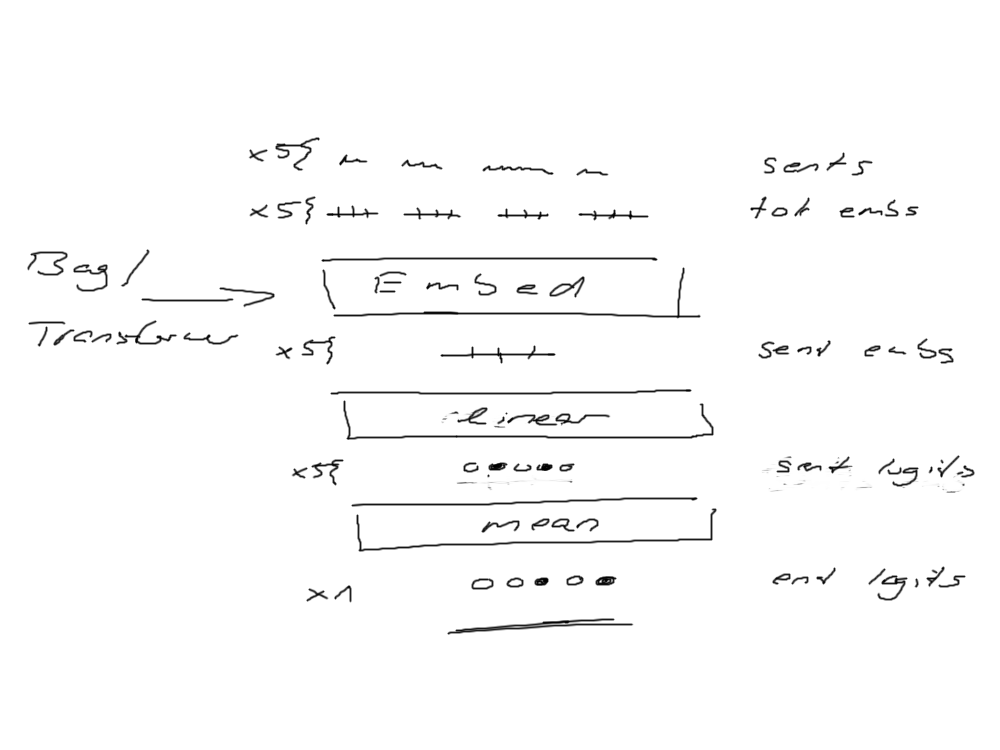
\includegraphics{4_approach/1_texter/1_simple_model/simple_architecture}
    \caption{Simple Texter Architecture; Each sentence is embedded and classified individually before the final pooling layer combines the results; "++++----" represents an embedding with positive and negative elements}
    \label{fig:4_approach/1_texter/1_simple_model/simple_architecture}
\end{figure}

several parts of it can be adjusted
Most notably, embedding the sentences can be performed using either static or contextual word embeddings.
chapter experiments shows performance difference
